\documentclass[11pt, aspectratio=169]{beamer}

\usepackage{amsmath}
\usepackage{booktabs}
\usepackage{color}
\usepackage{csquotes}
\usepackage{fontspec}

%%%%%%%%%%%%%%%%%%%%%%%%%%%%%%%%%%%%%%%%%%%%%%%%%%%%%%%%
% Theme
%%%%%%%%%%%%%%%%%%%%%%%%%%%%%%%%%%%%%%%%%%%%%%%%%%%%%%%%

\usetheme[progressbar=frametitle]{metropolis}
\metroset{block=fill}
\metroset{sectionpage=progressbar}
\usefonttheme{professionalfonts}
\usepackage{theme/beamercolorthememetropolisinria}

%%%%%%%%%%%%%%%%%%%%%%%%%%%%%%%%%%%%%%%%%%%%%%%%%%%%%%%%
% Syntax highlighting
%%%%%%%%%%%%%%%%%%%%%%%%%%%%%%%%%%%%%%%%%%%%%%%%%%%%%%%%

\usepackage{minted}
\definecolor{codebg}{rgb}{0.95, 0.955, 0.96}

\setminted[bash]{
    autogobble,
    baselinestretch=1.2,
    bgcolor=codebg,
    fontsize=\footnotesize,
    framesep=50mm,
    xleftmargin=1em,
    xrightmargin=1em,
}

\setminted[python]{
    autogobble,
    baselinestretch=1.2,
    bgcolor=codebg,
    fontsize=\footnotesize,
    framesep=50mm,
    xleftmargin=0.5em,
    xrightmargin=0.5em,
}

%%%%%%%%%%%%%%%%%%%%%%%%%%%%%%%%%%%%%%%%%%%%%%%%%%%%%%%%
% Bibliography
%%%%%%%%%%%%%%%%%%%%%%%%%%%%%%%%%%%%%%%%%%%%%%%%%%%%%%%%

\usepackage[
    style=alphabetic,
    maxbibnames=99,
    maxcitenames=99,
]{biblatex}
\addbibresource{refs.bib}

%%%%%%%%%%%%%%%%%%%%%%%%%%%%%%%%%%%%%%%%%%%%%%%%%%%%%%%%
% Footnotes
%%%%%%%%%%%%%%%%%%%%%%%%%%%%%%%%%%%%%%%%%%%%%%%%%%%%%%%%

\newcommand\blfootcite[1]{%
    \invisible<1>{%
        {\color{white} \footfullcite{#1}}%
    }%
}

\newcommand\blfootcitetext[1]{%
    \invisible<1>{%
        \addtocounter{footnote}{-1}% assumes a footnotemark
        {\color{white} \footfullcite{#1}}%
    }%
}

\newcommand\blfootnote[1]{%
  \begingroup
  \renewcommand\thefootnote{}%
  \footnote{#1}%
  \addtocounter{footnote}{-1}%
  \endgroup
}

\newcommand\blfootnotetext[1]{%
  \begingroup
  \footnotetext{#1}%
  \endgroup
}

%%%%%%%%%%%%%%%%%%%%%%%%%%%%%%%%%%%%%%%%%%%%%%%%%%%%%%%%
% Abbreviations
%%%%%%%%%%%%%%%%%%%%%%%%%%%%%%%%%%%%%%%%%%%%%%%%%%%%%%%%

\def\eg{{\emph{e.g.}}}
\def\etal{{\emph{et al.}}}
\def\ie{{\emph{i.e.}}}
\def\xid{\dot{\xi}}

%%%%%%%%%%%%%%%%%%%%%%%%%%%%%%%%%%%%%%%%%%%%%%%%%%%%%%%%
% Metadata
%%%%%%%%%%%%%%%%%%%%%%%%%%%%%%%%%%%%%%%%%%%%%%%%%%%%%%%%

\title{
    Reinforcement learning for legged robots
}

\author{\textbf{St\'ephane Caron}}
\date{October 13, 2023}
\institute{Inria--\'{E}cole normale sup\'{e}rieure}

\begin{document}

\maketitle

%%%%%%%%%%%%%%%%%%%%%%%%%%%%%%%%%%%%%%%%%%%%%%%%%%%%%%%%%%%%%%%%%%%%%%%%%%%%%%%%

\section*{Robots with policies trained by RL}

\begin{frame}{2020: Quadrupedal locomotion~\cite{lee2020}}
    \vspace{1.5em}
    \begin{figure}
        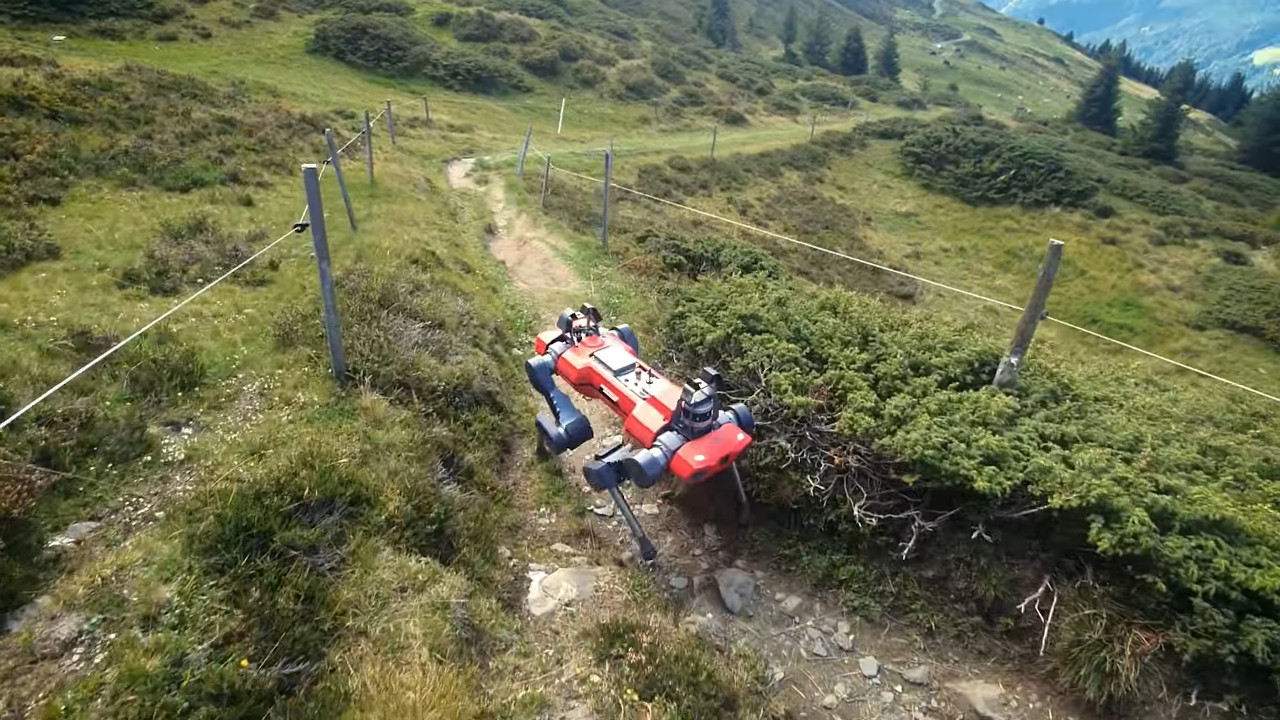
\includegraphics[height=5.5cm]{figures/hike-with-anymal.jpg}
    \end{figure}
    \begin{center}
        Teacher-student, residual reinforcement learning
    \end{center}
    \blfootnote{
        Video: \url{https://youtu.be/oPNkeoGMvAE}
    }
\end{frame}

\begin{frame}{2018: In-hand reorientation}
    \vspace{1.5em}
    \begin{figure}
        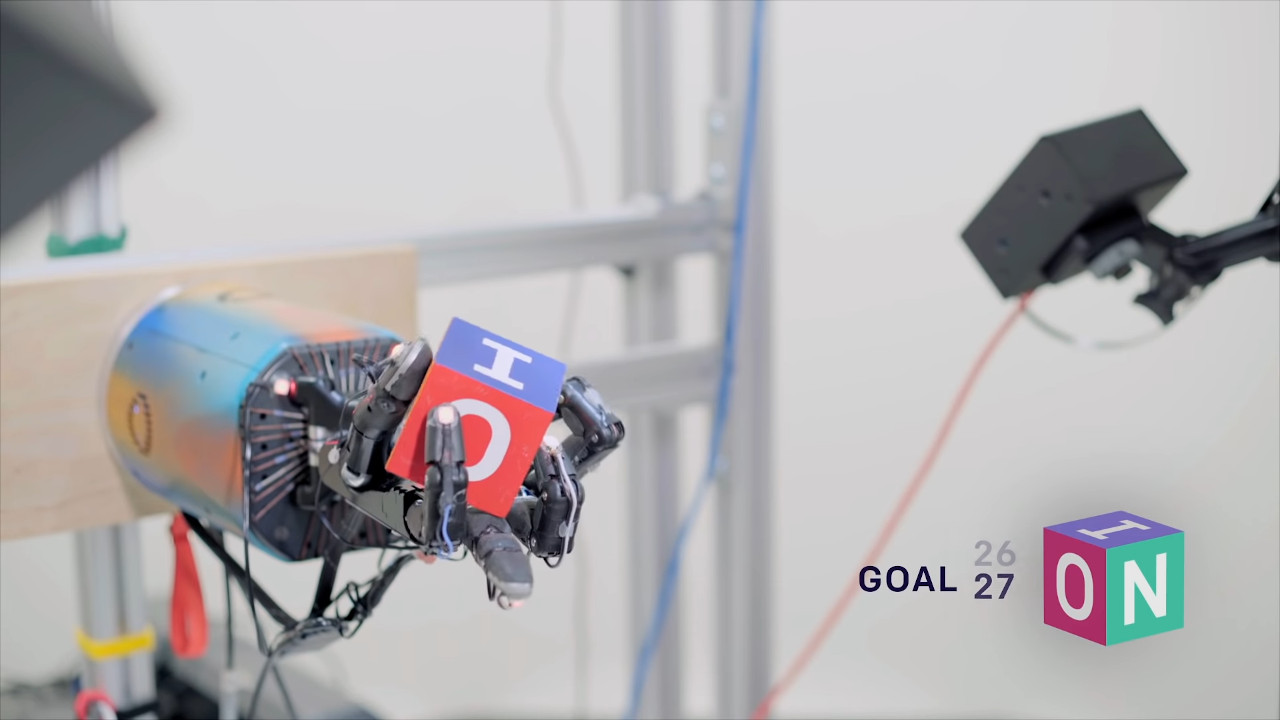
\includegraphics[height=5.5cm]{figures/in-hand-reorientation.jpg}
    \end{figure}
    \begin{center}
        Domain randomization, LSTM policy
    \end{center}
    \blfootnote{
        Video: \url{https://youtu.be/jwSbzNHGflM}
    }
\end{frame}

\begin{frame}{2010: Helicopter stunts}
    \vspace{1.5em}
    \begin{figure}
        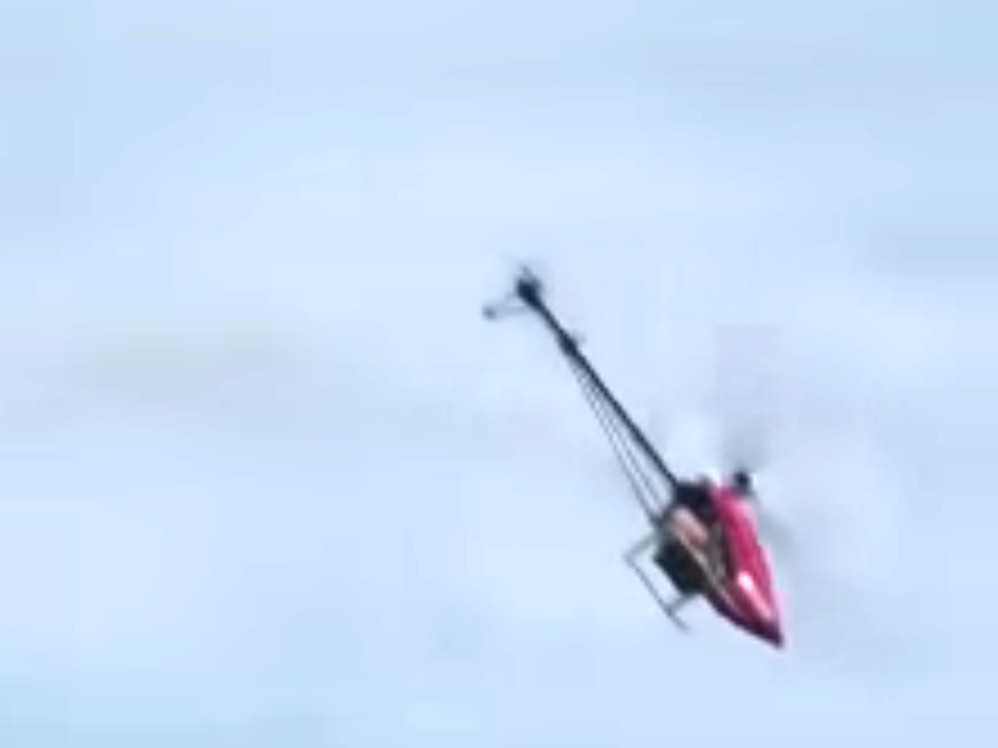
\includegraphics[height=3.5cm]{figures/helicopter-stunts.jpg}
    \end{figure}
    \begin{center}
        Autonomous Helicopter Aerobatics through Apprenticeship Learning~\cite{abbeel2010}
    \end{center}
    \blfootnote{
        Video: \url{https://youtu.be/M-QUkgk3HyE}
    }
\end{frame}

\begin{frame}{1997: Pendulum swing up~\cite{atkeson1997}}
    \vspace{1.5em}
    \begin{figure}
        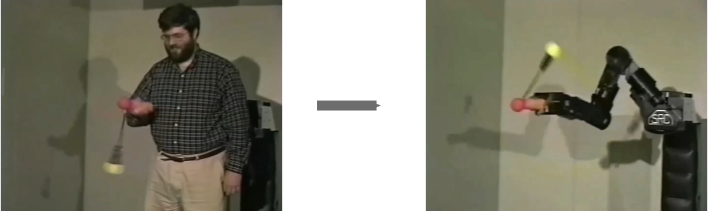
\includegraphics[height=3.5cm]{genfig/atkeson-demo.pdf}
    \end{figure}
    \blfootnote{
        Video: \url{https://youtu.be/g3I2VjeSQUM?t=294}
    }
\end{frame}

%%%%%%%%%%%%%%%%%%%%%%%%%%%%%%%%%%%%%%%%%%%%%%%%%%%%%%%%%%%%%%%%%%%%%%%%%%%%%%%%

\section*{Intro to reinforcement learning}

\begin{frame}{Scope}
    \begin{figure}
        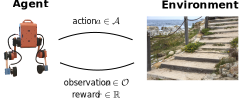
\includegraphics[height=5cm]{genfig/agent-environment.pdf}
    \end{figure}
\end{frame}

\begin{frame}{Rewards}
    \begin{figure}
        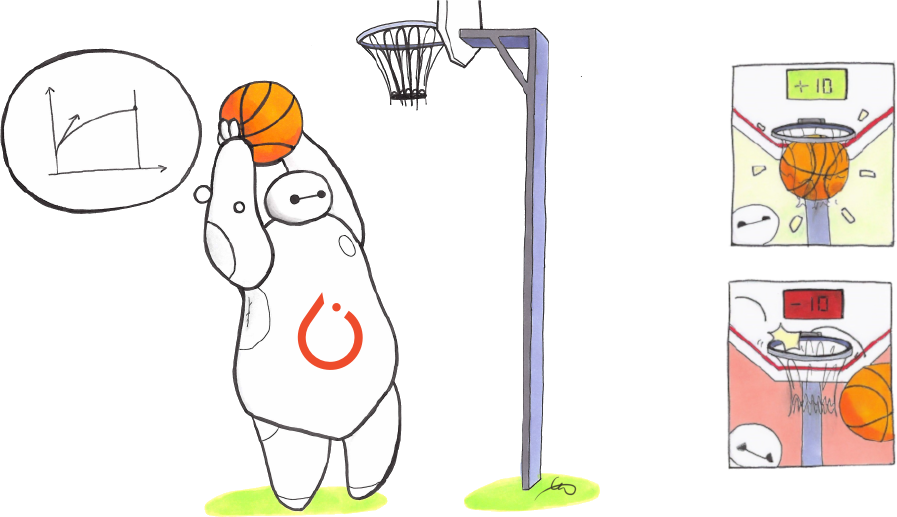
\includegraphics[height=5.5cm]{figures/stable-baselines3-logo.png}
    \end{figure}
    \blfootnote{
        Image credit: L. M. Tenkes, source: \url{https://araffin.github.io/post/sb3/}
    }
\end{frame}

\begin{frame}{Terminology}
    \begin{itemize}
        \item \textbf{State:} $s_t$, ground truth of the environment
        \item \textbf{Action:} $a_t$, computed
        \item \textbf{Model:} $s_{t+1} = f(s_t, a_t)$, how the environment evolves
            \begin{itemize}
                \item Deterministic: $s_{t+1} = f(s_t, a_t)$
                \item Stochastic: $s_{t+1} \sim p(\cdot | s_t, a_t)$
            \end{itemize}
        \item \textbf{Observation:} $o_t$, read from robot sensors
    \end{itemize}
\end{frame}

\begin{frame}{Terminology}
    \begin{itemize}
        \item \textbf{Reward:} $r_t$, often $r_t = r(s_t, a_t)$ or $r(s_t, a_t, s_{t+1})$
        \item \textbf{Return:} $G_t = \sum_t r_t$
    \end{itemize}
    For instance, for a trajectory $\tau = (s_0, a_0, s_1, a_1, \ldots, s_{N-1}, a_{N-1}, s_N)$:
    $$
    G_0 = \sum_{t = 0}^{N-1} r(s_t, a_t) + r_{\mathit{last}}(s_N)
    $$
\end{frame}

\begin{frame}{Terminology}
    \begin{table}
        \begin{tabular}{ll}
            \textbf{Reinforcement learning} & \textbf{Control theory} \\
            \hline
            State: $s_t$ & $x_t$ \\
            Observation: $o_t$ & $y_t$ \\
            Action: $a_t$ & Input: $u_t$ \\
            Reward: $r_t$ & Stage cost: $\ell(x_t, u_t)$ \\
            Return: $\max G_t = \sum_t r_t$ & Cost: $\min J = \sum_t \ell(x_t, u_t)$ \\
            Model: $s_{t+1} = f(s_t, a_t)$ & Dynamics: $x_{t+1} = f(x_t, u_t)$ \\
        \end{tabular}
    \end{table}
\end{frame}

\begin{frame}{Components of an RL algorithm}
    \begin{itemize}
        \item Policy: behavior function $a_t = \pi(o_t)$
        \item Value function: 
    \end{itemize}
\end{frame}

\begin{frame}{Optimal control and RL}
    ...
\end{frame}

\begin{frame}{Policy gradient theorem}
    ...
\end{frame}

\begin{frame}{The Gymnasium API}
    \begin{itemize}
        \item API for single-agent reinforcement learning environments
        \item Widespread, not necessarily the best one out there
    \end{itemize}
\end{frame}

\begin{frame}{Domain randomization}
    ...
\end{frame}

\begin{frame}{Reward vocabulary}
    Let $r_e$ denote the reward associated with an error function $e$:

    Motivation:
    \begin{itemize}
        \item Exponential: $r_e = \exp(-e^2)$
    \end{itemize}

    Penalization:
    \begin{itemize}
        \item Absolute value $r_e = -|e|$
        \item Squared value: $r_e = -e^2$
    \end{itemize}
\end{frame}

\begin{frame}{Environment bounds}
    \begin{figure}
        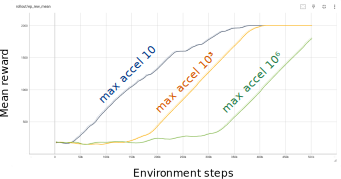
\includegraphics[width=\columnwidth]{genfig/max-accel.pdf}
    \end{figure}
\end{frame}

\begin{frame}{Caveat: stochastic}
    \begin{figure}
        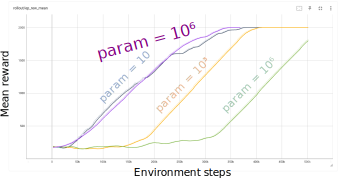
\includegraphics[width=\columnwidth]{genfig/max-accel-bis.pdf}
    \end{figure}
\end{frame}

\begin{frame}{Normalizing observations}
    \begin{itemize}
        \item Normalizing:
        \item Standardizing:
    \end{itemize}
\end{frame}

\begin{frame}{Normalizing observations}
    not always a good thing! see figure
\end{frame}

\begin{frame}{Other entries in the cookbook}
    \begin{itemize}
        \item Add a temporary reward $r_{bias}$, remove it once $r = \sum_i r_i$ reaches 50\% of the maximum reward (done \emph{e.g.} in~\cite{rudin2022advanced}).
    \end{itemize}
\end{frame}

\begin{frame}{That's all folks!}
    \vspace{2em}
    \begin{figure}
        \centering
        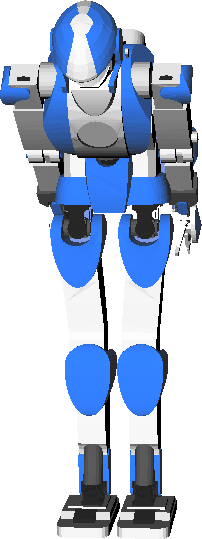
\includegraphics[height=10em]{genfig/thanks.pdf}
    \end{figure}
\end{frame}

%%%%%%%%%%%%%%%%%%%%%%%%%%%%%%%%%%%%%%%%%%%%%%%%%%%%%%%%%%%%%%%%%%%%%%%%%%%%%%%%

\section*{Bibliography}

\renewcommand*{\bibfont}{\footnotesize}
\setbeamertemplate{bibliography item}{\insertbiblabel}
\begin{frame}[allowframebreaks]{References}
    \printbibliography[heading=none]
\end{frame}

\section*{Templates}

\begin{frame}[fragile]{Python code}
    Load a robot description:
    \begin{minted}{python}
        from robot_descriptions.loaders.pinocchio import load_robot_description

        robot = load_robot_description("upkie_description")
    \end{minted}
    Visualize it:
    \begin{columns}
        \begin{column}{0.75\columnwidth}
            \begin{minted}{python}
                from pinocchio.visualize import MeshcatVisualizer

                robot.setVisualizer(MeshcatVisualizer())
                robot.initViewer(open=True)
                robot.loadViewerModel()
                robot.display(robot.q0)
            \end{minted}
        \end{column}
        \begin{column}{0.24\columnwidth}
            \begin{figure}
                \centering
                % \includegraphics[width=\columnwidth]{figures/upkie_description.png}
            \end{figure}
        \end{column}
    \end{columns}
    \blfootnote{
        Setup: \mintinline{bash}{pip install meshcat pin robot_descriptions}
    }
\end{frame}

\end{document}
